\documentclass{article}
\usepackage{amsmath, amssymb, amsthm, enumitem}
\usepackage{fullpage}
\usepackage{tikz}
\newtheorem{corollary}{Corollary}

\title{Discrete Mathematics 1 Lectures, Part 1}
\author{Tomasz Brengos}
\date{}

\begin{document}
\maketitle

\section{Counting (Combinatorics)}

Counting forms the basis of combinatorics. In these lectures we explore several counting rules, examples, and proofs.

\subsection{Rule of Sum (Addition Principle)}
If a set $S$ is partitioned into disjoint subsets,
\[
S = S_1 \cup S_2 \cup \cdots \cup S_k,
\]
then the total number of elements in $S$ is the sum of the number of elements in each subset:
\[
|S| = |S_1| + |S_2| + \cdots + |S_k|.
\]

\paragraph{Example:}  
Suppose we wish to count the number of ways to choose a subset of a set $X$ of size $u$, but we only consider subsets of a fixed size $k$. If we let $S$ be the family of all such subsets, then using the rule of sum by dividing the choices according to a distinguished element (say, whether a chosen element is included or not) we can count the subsets by summing over the possibilities. (This idea is used later in proofs for binomial coefficients and the power set.)

\paragraph{Theorem:}
\[
\binom{n}{k} = \binom{n-1}{k-1} + \binom{n-1}{k}
\]

\paragraph{Proof:}
Consider \( S = \binom{X}{k} \), the set of all subsets of \( X \) of size \( k \).  
Take any element \( a \in X \). Define:  
 \( S_1 \) as the subsets in \( S \) that contain \( a \) and  
 \( S_2 \) as the subsets in \( S \) that do not contain \( a \).  

Since every subset of \( S \) either contains \( a \) or does not, we see that \( S_1 \) and \( S_2 \) are disjoint and their union forms \( S \), i.e.,  
\[
S_1 \cup S_2 = S.
\]

By the rule of sum, we get:  
\[
|S| = |S_1| + |S_2|.
\]

Now,  
each subset in \( S_1 \) must contain \( a \), so we choose the remaining \( k-1 \) elements from \( X \setminus \{a\} \), which has \( n-1 \) elements. Thus, \( |S_1| = \binom{n-1}{k-1} \).  
Each subset in \( S_2 \) does not contain \( a \), so we choose all \( k \) elements from \( X \setminus \{a\} \). Thus, \( |S_2| = \binom{n-1}{k} \).  

Therefore,  
\[
\binom{n}{k} = |S| = |S_1| + |S_2| = \binom{n-1}{k-1} + \binom{n-1}{k}.
\]

\paragraph{Example:}  
Let \( S = \{ \triangle, \square, \circ \} \) and \( k = 2 \), choosing \( a = \circ \).  
Fixing \( \circ \) as one of the elements in the subset of size \( k \), we get:  
  \[
  S_1 = \{\{\circ, \triangle\}, \{\circ, \square\}\}.
  \]
Taking all subsets of size \( k \) without \( \circ \):  
  \[
  S_2 = \{\{\triangle, \square\}\}.
  \]
We have \( |S_1| = 2 \) and \( |S_2| = 1 \), so \( |S_1| + |S_2| = 3 \).  

\noindent On the other hand,  
\begin{align*}
\binom{3}{2} &= \frac{3!}{2!(3-2)!} = 3.
\end{align*}
Thus, \( |S| = |S_1| + |S_2| = 3 \), verifying the identity.  


\paragraph{}

\subsection{Rule of Product (Multiplication Principle)}
When an object is constructed by a sequence of choices, where:
\begin{itemize}[nosep]
    \item The first choice can be made in $a$ ways,
    \item The second in $b$ ways,
    \item $\ldots$
\end{itemize}
the total number of objects is the product:
\[
a \times b \times \cdots.
\]

\paragraph{Example:}  
A word of length $n$ over the binary alphabet $\{0,1\}$ is formed by choosing one of $2$ possibilities for each position. Hence, there are
\[
2^n
\]
possible words.

\subsection{Rule of Bijection}
If there exists a bijection (a one-to-one and onto mapping) between two sets $S$ and $T$, then they have the same number of elements:
\[
|S| = |T|.
\]

\paragraph{Example:}  
Consider the power set of a set $X$, denoted by $\mathcal{P}(X)$. There is a natural bijection between $\mathcal{P}(X)$ and the set of binary sequences of length $|X|$: for each subset $A \subseteq X$, assign the sequence $(a_1,a_2,\dots,a_n)$ where 
\[
a_i = \begin{cases} 
1, & \text{if } x_i \in A, \\
0, & \text{if } x_i \notin A.
\end{cases}
\]
This shows that 
\[
|\mathcal{P}(X)| = 2^{|X|}.
\]

\subsection{Counting in Two Ways}  

\paragraph{Rule of Counting in Two Ways}  
When two formulae enumerate the same quantity, they must be equal.  

\paragraph{Example:}  
\[
\sum_{i=1}^{n} i = \frac{n(n+1)}{2}
\]

\paragraph{Proof:}  
Consider a lattice grid of size \( (n+1) \times (n+1) \), defined as:  
\[
X = \{(i, j) \mid i, j \in \{1, 2, \dots, n+1\} \}.
\]  
Clearly, \( |X| = (n+1)^2 \).  

Now, partition \( X \) into three subsets:  
- \( X_1 \), the points strictly below the secondary diagonal.  
- \( X_2 \), the points strictly above the secondary diagonal.  
- \( X_3 \), the points on the secondary diagonal itself.  

Since these three sets form a partition, we have:  
\[
|X| = |X_1| + |X_2| + |X_3|.
\]  
Observing their sizes:  
\[
|X_1| = |X_2| = 1 + 2 + \dots + n, \quad |X_3| = n+1.
\]  
Thus,  
\[
(n+1)^2 = 2(1 + 2 + \dots + n) + (n+1).
\]  
Rearranging, we get:  
\[
1 + 2 + \dots + n = \frac{(n+1)^2 - (n+1)}{2} = \frac{n(n+1)}{2}.
\]

Hence, we have proven the formula:  
\[
\sum_{i=1}^{n} i = \frac{n(n+1)}{2}.
\]


\subsection{Binomial Coefficients and Permutations}
Let $X$ be a set with $|X| = n$.

\paragraph{Subsets:}  
The number of ways to choose a $k$-subset of $X$ is given by the binomial coefficient
\[
\binom{n}{k}.
\]

\paragraph{Permutations:}  
A \( k \)-permutation of a set \( X \) of size \( n \) is a \( k \)-word over the alphabet \( X \) whose entries are distinct.  

\paragraph{Theorem:}  
There are exactly  
\[
n (n-1) (n-2) \dots (n-k+1)
\]  
\( k \)-permutations of an \( n \)-set.  

\paragraph{Question:}  
How are \( k \)-permutations of an \( n \)-set related to \( k \)-subsets of an \( n \)-set?  

\paragraph{Answer:}  
The difference between a \( k \)-permutation and a \( k \)-subset is that a permutation is ordered, while a subset is not.  
To express a \( k \)-permutation in terms of a \( k \)-subset, we need to account for all possible arrangements of the elements, which is \( k! \).  
Thus,  
\[
\text{\( k \)-permutation} = \binom{n}{k} \cdot k!
\]
Expressing \( \binom{n}{k} \) as  
\[
\binom{n}{k} = \frac{n!}{k!(n-k)!}
\]  
we obtain:  
\[
\text{\( k \)-permutation} = \frac{n!}{(n-k)!}.
\]


\paragraph{Proof by Counting in Two Ways:}  
Count the number of $k$-permutations of an $n$-set in two ways:
\begin{enumerate}[label=(\arabic*)]
    \item Directly, by applying the rule of product:
    \[
    n \times (n-1) \times \cdots \times (n-k+1) = \frac{n!}{(n-k)!}.
    \]
    \item First choose a $k$-subset (in $\binom{n}{k}$ ways) and then arrange it (in $k!$ ways), giving
    \[
    \binom{n}{k} \cdot k!.
    \]
\end{enumerate}
Equate these two counts to obtain the relation.

\subsection{Binomial Theorem}
For any $x,y$ in a field and nonnegative integer $n$, the binomial theorem states:
\[
(x+y)^n = \sum_{k=0}^{n} \binom{n}{k} x^k y^{n-k}.
\]
\paragraph{Explanation:}  
This theorem is a direct consequence of counting the number of ways to choose $k$ copies of $x$ (and the remaining $n-k$ copies of $y$) when expanding the product.

\subsection{Multisets}  

\paragraph{Definition:}  
A multiset of a set \( X \) of size \( n \) is a function  
\[
m: X \to \mathbb{N}
\]
that assigns a non-negative integer to each element of \( X \), representing its multiplicity in the multiset.  

\paragraph{Example:}  
Let \( X = \{a, b, c\} \), and consider the multiset \( \{a, a, b\} \). Then, the function \( m \) is given by:  
\[
m(a) = 2, \quad m(b) = 1, \quad m(c) = 0.
\]  

\paragraph{Question:}  
What is the number of \( k \)-multisets of a set of size \( n \)?  

\paragraph{Theorem:}  
The number of all \( k \)-multisets of an \( n \)-set is  
\[
\binom{n+k-1}{k}.
\]  

\paragraph{Proof:}  
Let \( X \) be the set of all \( k \)-multisets of an \( n \)-set.  
Let \( Y \) be the set of all distributions of \( k \) identical objects into \( n \) buckets.  

\paragraph{Claim 1:}  
There is a bijection from \( X \) to \( Y \).  
Thus, by the rule of bijection, we have  
\[
|X| = |Y|.
\]  

\paragraph{Claim 2:}  
Let \( Z \) be the set of all binary sequences of length \( n+k-1 \) with exactly \( n-1 \) ones (or equivalently, \( k \) zeros).  
There is a bijection from \( Y \) to \( Z \).  
Hence,  
\[
|Y| = |Z| \Rightarrow |X| = |Z|.
\]  
Since the number of such binary sequences is given by  
\[
\binom{n+k-1}{k},
\]  
we conclude that  
\[
|X| = \binom{n+k-1}{k}.
\]


\subsection{Lattice Paths}
Consider an $m \times n$ grid with lattice points at the intersections.  
\paragraph{Problem:}  
How many paths are there from $(0,0)$ to $(m,n)$ if one may only move right or up?
\paragraph{Solution:}  
Every path consists of exactly $m$ right moves and $n$ up moves. Thus, a path can be represented as a sequence of $m+n$ moves, where we choose $n$ positions (out of $m+n$) for the up moves. Hence, the number of paths is:
\[
\binom{m+n}{n}.
\]

\paragraph{Bijection Explanation:}  
There is a bijection between the set of such lattice paths and the set of binary sequences of length $m+n$ with exactly $n$ ones (representing the up moves).

\section{Partitions and Stirling Numbers}
\subsection{Set Partitions}  
\paragraph{Definition:}  
A set \( \{ A_1, A_2, \dots, A_k \} \) of subsets of \( N \) forms a \emph{partition of} the set \( N \) if:
\[
A_i \neq \emptyset, \quad A_i \cap A_j = \emptyset \text{ for } i \neq j, \quad \text{and} \quad N = A_1 \cup A_2 \cup \dots \cup A_k.
\]
If a partition \( P \) of the set \( N \) is of size \( k \) then we say that \( P \) partitions \( N \) into \( k \) blocks. 
\paragraph{Example:}  
For \( N = \{1,2,3,4\} \), one partition into \( 2 \) blocks could be  
\[
\{\{1,3\}, \{2,4\}\}.
\]  
\emph{All possible partitions} of a set \( N \) are denoted by \( \Pi(N) \).

\subsection{Stirling Numbers of the Second Kind}
 \paragraph{Question:}  
How many \( k \)-partitions of an \( n \)-set are there?  
\paragraph{Answer:}  
Let \( S(n, k) \) (or \( \{n \; k\} \)) denote the answer to our question, called the \emph{Stirling number of the second kind}.  
We define the base cases as follows:  
\[
S(0,0) := 1, \quad S(0,k) := 0 \quad \text{for } k > 0.
\]  
\paragraph{Theorem:}  
The total number of set partitions of \( N \) is given by  
\[
|\Pi(N)| = \sum_{k=0}^{|N|} S(|N|, k).
\]  
\paragraph{Remark:}  
The quantity  
\[
B(|N|) := |\Pi(N)| = \sum_{k=0}^{|N|} S(|N|, k)
\]  
is called the \emph{Bell number}.
\paragraph{Example:}  
Let \( N = [5] = \{1,2,3,4,5\} \). List all possible 2-partitions of \( N \).  

Firstly, consider cases where the first subset contains only one element:  
\[
1 | 2\,3\,4\,5, \quad 2 | 1\,3\,4\,5, \quad 3 | 1\,2\,4\,5, \quad 4 | 1\,2\,3\,5, \quad 5 | 1\,2\,3\,4.
\]  

Now, consider cases where the first subset contains two elements:  
\[
1\,2 | 3\,4\,5, \quad 1\,3 | 2\,4\,5, \quad 1\,4 | 2\,3\,5, \quad 1\,5 | 2\,3\,4,
\]
\[
2\,3 | 1\,4\,5, \quad 2\,4 | 1\,3\,5, \quad 2\,5 | 1\,3\,4, \quad 3\,4 | 1\,2\,5, \quad 3\,5 | 1\,2\,4, \quad 4\,5 | 1\,2\,3.
\]  

Since we are only interested in the contents of the two subsets (not their arrangement or order), we do not list cases where the first subset has three or four elements, as these would be overcounting.  
For example, the partitions \( 1\,2 | 3\,4\,5 \) and \( 3\,4\,5 | 1\,2 \) are considered the same.  

Thus, all possible partitions have been listed, and their total number is 15. Therefore,  
\[
S(5,2) = 15.
\]

\paragraph{Note:}  
Stirling numbers consider objects that we distribute as distinct, the boxes (subsets) as identical, and the size of subsets as known. Due to this, in the example, we did not consider the cases \( 1\,2 | 3\,4\,5 \) and \( 3\,4\,5 | 1\,2 \) as distinct.  

Additionally, Bell's number counts all possible partitions, meaning the number of subsets \( k \) is not fixed but varies from \( 0 \) to \( |N| \). This concept may seem similar to multisets; however, Bell's number treats objects being distributed as distinct and the boxes(subsets) as identical, while multisets treat objects as identical and boxes as distinct.


\paragraph{Recurrence Relation:}  
These numbers satisfy the recurrence:
\[
S(n,k) = S(n-1,k-1) + k\, S(n-1,k).
\]
\paragraph{Proof:}  
Let \( N = [n] \) and \( P \) be the set of all \( k \)-partitions of \( N \). We observe that \( |P| = S(n, k) \), where \( S(n, k) \) denotes the Stirling number of the second kind.  

Consider an element \( x \in [n] \). Define the following subsets of \( P \):  
 \( X_1 \) consists of partitions in \( P \) where \( x \) forms a singleton block, i.e., one of the subsets \( A_i \) in the partition \( \{A_1, A_2, \dots, A_k\} \) is \( \{x\} \).  
 \( X_2 = P \setminus X_1 \), meaning \( X_2 \) consists of partitions where \( x \) is not a singleton block but instead belongs to one of the \( k \) subsets.  

Now, we compute their cardinalities:  
 Since \( X_1 \) consists of partitions where \( x \) is a singleton, the remaining \( n-1 \) elements must be partitioned into \( k-1 \) subsets. Thus,  
  \[
  |X_1| = S(n-1, k-1).
  \]  
 In \( X_2 \), the element \( x \) is assigned to one of the \( k \) subsets after partitioning the remaining \( n-1 \) elements into \( k \) subsets. Thus,  
  \[
  |X_2| = k \cdot S(n-1, k).
  \]  

By the rule of sum,  
\[
S(n, k) = |X_1| + |X_2| = S(n-1, k-1) + k \cdot S(n-1, k).
\]
This completes the proof.

\subsection{Counting Maps}

\paragraph{Setup:}
Consider two finite sets \(N\) and \(R\) of sizes \(n\) and \(r\) respectively. We want to answer three main questions about the functions from \(N\) to \(R\): 

\paragraph{Q1: How many functions from \(N\) to \(R\) are there?}
\paragraph{Answer:} 
Each of the \(n\) elements of \(N\) can be mapped to any of the \(r\) elements of \(R\). Hence, there are \(r^n\) possible functions in total.

\paragraph{Q2: How many injective (one-to-one) functions from \(N\) to \(R\)?}
\paragraph{Answer:} 
To build an injective function, choose a distinct image in \(R\) for each element of \(N\). Thus, the number of injective functions is
\[
r \times (r - 1) \times (r - 2) \times \cdots \times (r - n + 1)
= \frac{r!}{(r - n)!}.
\]

\paragraph{Q3: How many surjective (onto) functions from \(N\) to \(R\)?}
\paragraph{Answer:}
A function \(f : N \to R\) is surjective if every element of \(R\) has a nonempty preimage. Equivalently, the sets 
\[
f^{-1}(y_1), \quad f^{-1}(y_2), \quad \dots, \quad f^{-1}(y_r)
\]
form a partition of \(N\) into \(r\) nonempty blocks. Since there are \(S(n,r)\) ways to partition \(N\) into \(r\) nonempty subsets (where \(S(n,r)\) is the Stirling number of the second kind), and each partition can be labeled in \(r!\) ways (assigning each of the \(r\) blocks to a different \(y_i \in R\)), the total number of surjections is
\[
\text{Sur}(n, r) = r! \cdot S(n, r)
\]

\paragraph{Corollary:}
Let \(N\) and \(R\) be finite sets with \(|N| = n\) and \(|R| = r\). Then the total number of functions from \(N\) to \(R\) can be expressed as
\[
| \mathrm{Map}(N, R) | \;=\; r^n \;=\; \sum_{k=0}^{r} \binom{r}{k} \; k! \; S(n,k).
\]


\subsection{Number Partitions}

\textbf{Definition.} A \emph{number partition} of \(n\in\mathbb{N}\) is an expression
\[
n = \lambda_1 + \lambda_2 + \cdots + \lambda_k,
\]
where
\[
\lambda_1 \ge \lambda_2 \ge \cdots \ge \lambda_k \ge 1.
\]

\medskip

\textbf{Example.} List all possible different number partitions of \(n=5\) into two summands:
\[
5 = 4+1 \quad \text{and} \quad 5 = 3+2.
\]

\medskip

\textbf{Question.} How many \(k\)-partitions of \(n\) are there?

\medskip

\textbf{Answer.} Define
\[
P(n,k)=\Bigl\{ (\lambda_1,\dots,\lambda_k)\,\Big|\, n=\lambda_1+\lambda_2+\cdots+\lambda_k,\; \lambda_1\ge\lambda_2\ge\cdots\ge\lambda_k\ge1 \Bigr\},
\]
and let
\[
p(n,k)=|P(n,k)|.
\]
Moreover, set
\[
P(n)=\bigcup_{k=1}^{n} P(n,k) \quad\text{and}\quad p(n)=|P(n)|.
\]
An immediate observation is that
\[
p(n)=\sum_{k=0}^{n} p(n,k).
\]

\medskip

\textbf{Example.} List all possible different number partitions of \(n=5\):
\[
P(5)=\Bigl\{\{5\},\, \{4,1\},\, \{3,2\},\, \{3,1,1\},\, \{2,2,1\},\, \{2,1,1,1\},\, \{1,1,1,1,1\}\Bigr\},
\]
with, for instance,
\[
P(5,1)=\{ \{5\}\},\quad P(5,2)=\{\{4,1\},\{3,2\}\},\quad P(5,3)=\{\{3,1,1\},\{2,2,1\}\},
\]
\[
P(5,4)=\{\{2,1,1,1\}\},\quad P(5,5)=\{\{1,1,1,1,1\}\}.
\]

\medskip

To derive recursive formulas for \(p(n)\) and \(p(n,k)\), we introduce the notation
\[
p(n,\le k)\stackrel{\text{def}}{=} |P(n,\le k)|,\quad\text{where}\quad P(n,\le k)=\bigcup_{i=1}^{k} P(n,i).
\]
\begin{itemize}
  \item \textbf{Observation 1:} \(P(n,\le n)=P(n)\) and hence \(p(n,\le n)=p(n)\).
  \item \textbf{Observation 2:} 
  \[
  p(n,\le k)=\sum_{i=1}^{k} p(n,i)=p(n,1)+p(n,2)+\cdots+p(n,k).
  \]
\end{itemize}

\bigskip

\textbf{Theorem.} There is a bijection
\[
\Phi\colon P(n,k) \longrightarrow P(n-k,\le k),
\]
defined as follows.

\medskip

Represent a partition
\[
\lambda=(\lambda_1,\lambda_2,\dots,\lambda_k)\in P(n,k)
\]
by its Ferrers diagram drawn in the standard way (with the largest row on top). In this diagram, the top row has \(\lambda_1\) cells, the second row has \(\lambda_2\) cells, and so on.

\medskip

\textbf{Explanation of the Mapping.}  
Our goal is to relate partitions of \(n\) into exactly \(k\) parts to partitions of \(n-k\) with at most \(k\) parts. Notice that if we subtract \(1\) from each part \(\lambda_i\), then
\[
n = \lambda_1+\lambda_2+\cdots+\lambda_k \quad \Longrightarrow \quad n-k = (\lambda_1-1)+(\lambda_2-1)+\cdots+(\lambda_k-1).
\]
Graphically, subtracting \(1\) from a part corresponds to removing one cell from its corresponding row. Since the Ferrers diagram is left-justified, every row begins with a cell in the leftmost column. Thus, removing the entire leftmost column is equivalent to subtracting \(1\) from each \(\lambda_i\). In this way, the original diagram representing a partition of \(n\) with \(k\) parts is transformed into a diagram representing a partition of \(n-k\) that has at most \(k\) parts (some rows may vanish if \(\lambda_i=1\)).

\medskip

\textbf{Example.} Consider the partition \((\lambda_1,\lambda_2,\lambda_3)=(4,2,1)\) of \(n=7\) into \(3\) parts. Its Ferrers diagram is:

\begin{center}
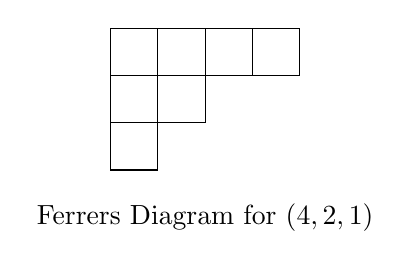
\begin{tikzpicture}[scale=0.6]
  % Ferrers diagram for (4,2,1)
  % Top row: 4 cells (\(\lambda_1=4\))
  \draw (0,0) rectangle (1,1);
  \draw (1,0) rectangle (2,1);
  \draw (2,0) rectangle (3,1);
  \draw (3,0) rectangle (4,1);
  % Second row: 2 cells (\(\lambda_2=2\))
  \draw (0,-1) rectangle (1,0);
  \draw (1,-1) rectangle (2,0);
  % Third row: 1 cell (\(\lambda_3=1\))
  \draw (0,-2) rectangle (1,-1);
  
  \node at (2,-3) {Ferrers Diagram for \((4,2,1)\)};
\end{tikzpicture}
\end{center}

Removing the leftmost column yields:

\begin{center}
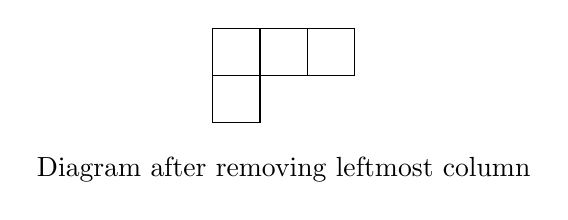
\begin{tikzpicture}[scale=0.6]
  % Diagram after removing the leftmost column from (4,2,1)
  % Top row now has 3 cells
  \draw (0,0) rectangle (1,1);
  \draw (1,0) rectangle (2,1);
  \draw (2,0) rectangle (3,1);
  % Second row now has 1 cell
  \draw (0,-1) rectangle (1,0);
  % Third row now has 0 cells (and is omitted)
  
  \node at (1.5,-2) {Diagram after removing leftmost column};
\end{tikzpicture}
\end{center}

The new diagram represents the partition \((3,1)\), which is a partition of \(7-3=4\) (since there were \(k=3\) rows, and we removed one cell per row). Note that \((3,1)\) is an element of \(P(4,\le 3)\).

\medskip

\textbf{Justification of Bijectivity.}  
The mapping
\[
\Phi\colon (\lambda_1,\lambda_2,\dots,\lambda_k) \mapsto (\lambda_1-1,\lambda_2-1,\dots,\lambda_k-1)
\]
is invertible. Given any partition \(\mu\) in \(P(n-k,\le k)\) (which has at most \(k\) parts), we can reconstruct a unique partition in \(P(n,k)\) by adding \(1\) to each part and, if necessary, appending enough parts equal to \(1\) so that the total number of parts becomes exactly \(k\). In other words, the inverse mapping \(\Phi^{-1}\) is defined by:
\[
\Phi^{-1}\colon \mu = (\mu_1,\mu_2,\dots,\mu_r) \mapsto (\mu_1+1,\mu_2+1,\dots,\mu_r+1,\underbrace{1,1,\dots,1}_{k-r \text{ times}}),
\]
with \(r\le k\). It is straightforward to check that \(\Phi\) and \(\Phi^{-1}\) are mutual inverses. Thus, the mapping \(\Phi\) is a bijection, and we have the relation:
\[
p(n,k)=|P(n,k)| = |P(n-k,\le k)| = p(n-k,\le k).
\]

\medskip

This bijective correspondence is the key step in obtaining a recursive formula for \(p(n,k)\).

\begin{corollary}
For all integers \(n\ge k\ge 1\), we have
\[
p(n,k) = p(n-k,\le k)
      = p(n-k,1) + p(n-k,2) + \cdots + p(n-k,k-1) + p(n-k,k).
\]
That is, the total number of \(k\)-partitions of \(n\) can be split into partitions of \(n-k\) with at most \(k\) parts:
\[
p(n,k) = p(n-k,\le k-1) + p(n-k,k).
\]
Moreover, since
\[
p(n-k,\le k-1)=p((n-k)+(k-1),k-1)=p(n-1,k-1),
\]
we obtain the recurrence relation
\[
p(n,k)=p(n-1,k-1)+p(n-k,k).
\]
\end{corollary}




\section{Inclusion-Exclusion Principle}
Let $A_1, A_2, \dots, A_n$ be finite sets. Then the size of their union is given by:
\[
\left|\bigcup_{i=1}^n A_i\right| = \sum_{i=1}^n |A_i| - \sum_{1 \le i < j \le n} |A_i \cap A_j| + \sum_{1 \le i < j < k \le n} |A_i \cap A_j \cap A_k| - \cdots + (-1)^{n-1} |A_1 \cap A_2 \cap \cdots \cap A_n|.
\]

\paragraph{Proof Outline:}  
Each element that belongs to exactly $t$ of the sets $A_i$ is counted $\binom{t}{1}$ times in the first summation, subtracted $\binom{t}{2}$ times in the second, and so on. The alternating sum ensures that each element is counted exactly once.

\section{Permutations and Derangements}

\subsection{Permutations}
A permutation of an $n$-set is an arrangement of its elements. There are
\[
n!
\]
possible permutations.

\subsection{Derangements}
A \emph{derangement} is a permutation in which no element appears in its original position.  
\paragraph{Counting Derangements:}  
The number of derangements of an $n$-set, denoted $D(n)$, can be computed by:
\[
D(n) = n! \sum_{k=0}^{n} \frac{(-1)^k}{k!}.
\]
\paragraph{Proof using Inclusion-Exclusion:}  
Define, for each $i$, the set
\[
A_i = \{\text{permutations in which the } i\text{-th element is fixed}\}.
\]
Then, the number of derangements is the total number of permutations minus those that have at least one fixed point. Applying the inclusion-exclusion principle yields:
\[
D(n) = n! - \binom{n}{1}(n-1)! + \binom{n}{2}(n-2)! - \cdots + (-1)^n \binom{n}{n}0!.
\]
This simplifies to the formula above.

\section{Functions Between Sets}

Let $N$ and $R$ be sets with $|N| = n$ and $|R| = r$.

\begin{enumerate}[label=(\roman*)]
    \item \textbf{Total Functions:}  
    The number of functions from \( N \) to \( R \) is  
    \[
    r^n.
    \]  
    Explanation: For every element in \( N \), there are \( |R| = r \) possible values in \( R \). Thus, for the first element, there are \( r \) choices, for the second element, there are \( r \) choices, and so on.  
    Applying the rule of product, the total number of functions is \( r^n \).

    \item \textbf{Injective Functions:}  
    When \( r \geq n \), an injective function (one-to-one) from \( N \) to \( R \) can be chosen by assigning distinct images to the \( n \) elements.  

    If a function is injective, then for each value in the range there is only one corresponding argument. This means that function values cannot repeat, ensuring that \( x_1 \neq x_2 \) implies \( f(x_1) \neq f(x_2) \).  

    Since there are \( |R| = r \) choices for the first argument, \( r-1 \) choices for the second, \( r-2 \) for the third, and so on, applying the rule of product, the number of injective functions from \( N \) to \( R \) is:  
    \[
    r \cdot (r-1) \cdots (r-n+1) = \frac{r!}{(r-n)!}.
    \]
    \item \textbf{Surjective Functions:}  
    A function is surjective (onto) if every element in \( R \) has a pre-image in \( N \), meaning every element in \( R \) is an image of some element in \( N \).  
    Consider a surjection \( f: N \to R = \{y_1, y_2, \dots, y_r\} \). We observe that the preimages \( f^{-1}(y_1), f^{-1}(y_2), \dots, f^{-1}(y_r) \) form a partition of \( N \) into \( r \) non-empty subsets, as each element \( y_i \) in \( R \) corresponds to one or more elements from \( N \).  
    The number of ways to partition \( N \) into \( r \) parts is given by the Stirling number \( S(n, r) \), and since we can permute the \( r \) elements in \( R \) in \( r! \) ways, the total number of surjective functions from \( N \) to \( R \) is:  
    \[
    r! \, S(n, r),
    \]
    where \( S(n, r) \) is the Stirling number of the second kind, counting the ways to partition \( N \) into \( r \) non-empty subsets.

\end{enumerate}

\paragraph{Example:}  
For \( N = \{1, 2, 3\} \) and \( R = \{y_1, y_2\} \):
\begin{itemize}[nosep]
    \item[] Here \( |N| = 3 \) and \( |R| = 2 \).
    \item Total functions: $2^3 = 8$.
    \item Injective functions: Not possible since $|R|<|N|$.
    \item Surjective functions: Consider all possible surjective functions:

 \( f_1: \{1, 2\} \mapsto y_1, 3 \mapsto y_2 \)
- Another possible permutation for this partition: \( f_2: \{1, 2\} \mapsto y_2, 3 \mapsto y_1 \)
 \( f_3: \{2, 3\} \mapsto y_1, 1 \mapsto y_2 \)
- Another possible permutation for this partition: \( f_4: 1 \mapsto y_1, \{2, 3\} \mapsto y_2 \)
 \( f_5: \{1, 3\} \mapsto y_1, 2 \mapsto y_2 \)
- Another possible permutation for this partition: \( f_6: 2 \mapsto y_1, \{1, 3\} \mapsto y_2 \)

So, we have 6 surjective functions. Using the formula for surjective functions, we first find the Stirling number \( S(3, 2) = 3 \), which corresponds to the number of partitions without considering permutations. Then, accounting for the permutations of the \( r = 2 \) elements in \( R \), we compute:
\[
2! \cdot S(3, 2) = 2! \cdot 3 = 6,
\]
which matches the number of surjective functions we listed.
\end{itemize}

\section*{Additional Examples and Proofs from the Notes}

\subsection*{Example on Counting Words}
Let $S$ be the set of all words of length $n$ over the alphabet $\{0,1\}$. By the rule of product, each letter has 2 choices, and hence
\[
|S| = 2^n.
\]
Furthermore, if one wants to count the number of words with a given number of zeros and ones, one uses the binomial coefficient.

\subsection*{Example on Bijections for Power Sets}
Consider a set $X = \{x_1, x_2, \dots, x_n\}$. Each subset of $X$ can be represented by an $n$-tuple of 0's and 1's. The mapping that sends each subset to its corresponding binary vector is a bijection. This proves that
\[
|\mathcal{P}(X)| = 2^n.
\]

\subsection*{Proof of the Recurrence for Stirling Numbers}
Given an $n$-set, consider the addition of a new element $x$. When partitioning the set into $k$ blocks, either:
\begin{itemize}[nosep]
    \item $x$ forms a block by itself (which gives $S(n-1,k-1)$ partitions), or
    \item $x$ is added to one of the $k$ blocks of a partition of the remaining $n-1$ elements (which gives $k\, S(n-1,k)$ partitions).
\end{itemize}
Thus, we obtain
\[
S(n,k) = S(n-1,k-1) + k\, S(n-1,k).
\]

\subsection*{Proof of Derangements using Inclusion-Exclusion}
For the set $N=\{1,2,\ldots,n\}$, define
\[
A_i = \{\sigma \in S_n \mid \sigma(i) = i\}.
\]
Then, by the inclusion-exclusion principle,
\[
D(n) = n! - \sum_{i} |A_i| + \sum_{i<j} |A_i \cap A_j| - \cdots + (-1)^n |A_1 \cap \cdots \cap A_n|.
\]
Since $|A_i| = (n-1)!$, $|A_i \cap A_j| = (n-2)!$, and in general
\[
|A_{i_1} \cap \cdots \cap A_{i_k}| = (n-k)!,
\]
we have:
\[
D(n) = n! \left[ 1 - \frac{1}{1!} + \frac{1}{2!} - \cdots + (-1)^n \frac{1}{n!} \right].
\]

\end{document}

